%% Packages initialisation
\documentclass[10pt,compress]{beamer}
\usepackage[utf8]{inputenc}               % Enable UTF-8 compatible typing
\usepackage{hyperref}                     % Interactive PDF
\usepackage{mathtools}                    % Displaying math formulas etc.
\usepackage{tikz}                         % Drawing
\usetikzlibrary{trees}
\usetikzlibrary{calc}
\usepackage{listings}                     % Source code listings

\useinnertheme[sectionpage=none]{metropolis}
\useoutertheme[numbering=fraction]{metropolis}
\usetheme[everytitleformat=regular]{m}
\metroset{block=fill}
%\metroset[outer/number=fraction]

%% Hide navigation buttons
\beamertemplatenavigationsymbolsempty

%% Configure lstlisting environment
\lstdefinestyle{compact}{
    basicstyle=\ttfamily\tiny,
    breakatwhitespace=false,         
    breaklines=true,                 
    captionpos=b,                    
    keepspaces=true,                 
    numbers=none,                    
    numbersep=5pt,                  
    showspaces=false,                
    showstringspaces=false,
    showtabs=false,                  
    tabsize=2,
    escapeinside={(*}{*)}
}

\lstdefinestyle{spacey}{
    basicstyle=\ttfamily\small,
    breakatwhitespace=false,         
    breaklines=true,                 
    captionpos=b,                    
    keepspaces=true,                 
    numbers=none,                    
    numbersep=5pt,                  
    showspaces=false,                
    showstringspaces=false,
    showtabs=false,                  
    tabsize=2,
    escapeinside={(*}{*)}
}

\lstset{style=compact}

%% "Defined as" macro
\newcommand\defas{\mathrel{\overset{\makebox[0pt]{\mbox{\normalfont\tiny\sffamily def}}}{=}}}

%% Meta information
\author{Daniel Hillerström\\\footnotesize{\href{mailto:daniel.hillerstrom@ed.ac.uk}{daniel.hillerstrom@ed.ac.uk}\\\href{http://homepages.inf.ed.ac.uk/s1467124/}{http://homepages.inf.ed.ac.uk/s1467124/}}}
\title{Programming with Effect Handlers in Links}
\subtitle{\textit{PLInG, Autumn 2015, University of Edinburgh}}
\institute[University of Edinburgh]{School of Informatics\\The University of Edinburgh}
\date{\today}

%% Load slides
\begin{document}
% Front slide
\begin{frame}
  \titlepage
\end{frame}

% Load subsequent slides
\section{Project description}
\begin{frame}[fragile]
  \frametitle{Project description}
  \begin{block}{Motivation}
    \begin{itemize}
      \item Monads are great abstractions for programming with \emph{explicit} effects.\\
            But in general monads do not compose.
      \item Monad Transformers (MT) provide compositionality for monads.\\
            But MTs impose an implicit ordering on effects.
    \end{itemize}
  \end{block}    
  \begin{block}{Problem statement}
    \emph{How may we obtain modular, composable and unordered effects?}
  \end{block}
  \uncover<2->{
    Answer: Handlers for algebraic effects using row polymorphism!}
\uncover<3->{
 \begin{block}{Project aim}
   Provide an implementation of first-class effect handlers in the web-oriented functional programming language Links \cite{Links}.
 \end{block}
}
% \begin{block}{}
%   \begin{columns}
%     \begin{column}{.5\textwidth}
%       Phonebook example using monads
%       \begin{lstlisting}
% askNameAndNumber :: IO (Maybe (String,String))
% askNameAndNumber  = do
%   putStr "Enter your name> "
%   name    <- getLine
%   putStr "Enter your number> "
%   number  <- getLine
%   if isValid number
%     then (*\alert<2->{return \$ Just (name,number)}*)
%     else (*\alert<2->{return \$ Nothing}*)

% isValid :: String -> Bool
% isValid = all isDigit
%       \end{lstlisting}
%     \end{column}
%     \begin{column}{.5\textwidth}
%       Phonebook example using MTs
% \begin{lstlisting}
% askNameAndNumberT :: MaybeT IO (String,String)
% askNameAndNumberT = do
%   (*\alert<3->{lift}*) $ putStr "Enter your name> "
%   name   <- lift getLine
%   (*\alert<3->{lift}*) $ putStr "Enter your number> "
%   number <- getValidNumber
%   return (name,number)
  

% getValidNumber :: MaybeT IO String
% getValidNumber = do num <- lift getLine
%                     guard (isValid num)
%                     return num
% \end{lstlisting}
%     \end{column}
%   \end{columns}
% \end{block}
\end{frame}

% \begin{frame}
%   \frametitle{Project description (II)}
%   \begin{block}{Problem statement}
%     \emph{How may we obtain modular, composable and unordered effects?}
%   \end{block}
%   \uncover<2->{
%     Answer: Handlers for algebraic effects!}
% \uncover<3->{
%  \begin{block}{Project aim}
%    Provide an implementation of first-class effect handlers in the web-oriented functional programming language Links \cite{Links}.
%  \end{block}
% }
% \end{frame}

% \begin{frame}
%  \frametitle{Related work}
%  A handful of implementations already exists:
%  \begin{itemize}
%    \item Eff -- looks and feels like OCaml.
%    \item Haskell libraries, e.g.\small{ \href{http://homepages.inf.ed.ac.uk/slindley/papers/handlers.pdf}{\texttt{effect-handlers}}, \href{http://www.cs.ox.ac.uk/people/nicolas.wu/papers/Scope.pdf}{\texttt{scoped-handlers}}, \href{http://homepages.inf.ed.ac.uk/slindley/papers/frankly-draft-march2014.pdf}{\texttt{Frank}}}.
%    \item Idris library \href{http://eb.host.cs.st-andrews.ac.uk/drafts/effects.pdf}{\small\texttt{Effects}}.
%  \end{itemize}
%  How does our work differ from the aforementioned?
%  \begin{itemize}
%    \item Shortcoming: Limited effect polymorphism.
%    \item We propose, along the lines of Kammar et al. \cite{Kammar2013}, an implementation using row polymorphism.
%  \end{itemize}
% \end{frame}
\section{Effects and handlers}
\begin{frame}
  \frametitle{Effects and handlers}
  \begin{block}{Algebraic effect}
    An effect\footnote{We are assuming the free algebra, i.e. the equationless theory} is a collection of abstract operations, e.g. 
    $\{ Op_i : a_i \to b_i \}$
  \end{block}
  \begin{block}{Abstract computation}
    An abstract computation is composed from abstract operations.
  \end{block}

  \begin{block}{Handler}
    A handler is an interpreter. It instantiates an abstract computation with a concrete implementation.
  \end{block}
\end{frame}

\begin{frame}[fragile]
  \frametitle{Effects as computation trees \cite{Lindley14}}
Operation $\textsf{Choose} : () \to \texttt{Bool}$.

\vspace{0.5cm}
Picture the CPS term $\textsf{Choose}_{()}(\textsf{Choose}_{()}(2,4),\textsf{Choose}_{()}(8,16))$, e.g.
\vspace{0.5cm}
\begin{center}
\begin{tikzpicture}[level distance=1.5cm,
level 1/.style={sibling distance=3.5cm},
level 2/.style={sibling distance=1cm}]
%\tikzstyle{every node}=[circle,draw]

\node (Root) [blue,rectangle] {Choose ()}
    child { node[blue] (q0) {Choose ()} 
      child { node[draw=none] (q00) {2}
      }
      child { node[draw=none] (q01) {4} 
      }
      edge from parent node [draw=none,left,xshift=-2.0,yshift=2.0] {true}
    }
    child { node [blue] (q1) {Choose ()}
      child { node[draw=none] (q10) {8}
      }
      child { node[draw=none] (q11) {16}       
      }
      edge from parent node [draw=none,right,xshift=2.0,yshift=2.0] {false}
    };

\only<2-2>{\draw[->,red,rounded corners,dashed,line width=0.7pt]
    ($(Root) +(-1.0,0.2)$) --
    ($(q0) +(-1.0,0.4)$) --
    ($(q00) +(-0.3,0.0)$);}

\only<3-3>{\draw[->,red,rounded corners,dashed,line width=0.7pt]
    ($(Root) +(1.0,0.2)$) --
    ($(q1) +(1.0,0.4)$) --
    ($(q10) +(1.3,0.0)$);}

\only<4-5>{\draw[->,red,rounded corners,dashed,line width=0.7pt]
    ($(Root) +(-1.0,0.2)$) --
    ($(q0) +(-1.0,0.4)$) --
    ($(q00)  +(-0.5,0.0)$) --
    ($(q00)  +(-0.4,-0.35)$) --
    ($(q00)  +(0.0,-0.5)$) --
    ($(q00)  +(0.4,-0.35)$) --
    ($(q00)  +(0.5,0.0)$) --
    ($(q0)  +(-0.005,-0.3)$) --
    ($(q01)  +(-0.35,-0.35)$) --
    ($(q01)  +(0.0,-0.45)$) --
    ($(q01)  +(0.35,-0.35)$) --
    ($(q01)  +(0.4,0.0)$) --
    ($(q0)   +(1.0,0.5)$) --
    ($(Root) +(-0.3,-0.4)$) --
    ($(q1)  +(-0.8,-0.1)$) --
    ($(q10)  +(-0.5,0.0)$) --
    ($(q10)  +(-0.4,-0.35)$) --
    ($(q10)  +(0.0,-0.5)$) --
    ($(q10)  +(0.4,-0.35)$) --
    ($(q10)  +(0.5,0.0)$) --
    ($(q1)  +(-0.005,-0.3)$) --
    ($(q11)  +(-0.35,-0.35)$) --
    ($(q11)  +(0.0,-0.45)$) --
    ($(q11)  +(0.35,-0.35)$) --
    ($(q11)  +(0.4,0.0)$);}
\end{tikzpicture}
\end{center}
\only<1-1>{How should we interpret this computation?}
\only<2-2>{$\Rightarrow$ $2 : \texttt{Int}$ (Strictly positive)}
\only<3-3>{$\Rightarrow$ $16 : \texttt{Int}$ (depressingly pessimistic)}
\only<4-4>{How about this?}
\only<5-5>{$\Rightarrow [2,4,8,16] : [\texttt{Int}]$}
\end{frame}

\begin{frame}
  \frametitle{A game with sticks}
  \begin{center}
    \begin{figure}
      \includegraphics[scale=0.3]{sticks.jpg}
    \end{figure}
  \end{center}
  Set-up
  \begin{itemize}
    \item Two players: Alice and Bob; Alice always starts.
    \item One heap of $n$ sticks.
    \item Turn-based. Each player take between 1-3 sticks.
    \item The one, who takes the last stick, wins.
  \end{itemize}
We'll demonstrate how to encode strategic behaviour, compute game data, and cheat using handlers.
\end{frame}

\begin{frame}
  \frametitle{Game tree generated by \texttt{mtGen} with $n = 3$}
\begin{center}
\begin{tikzpicture}[level distance=1.5cm,
level 1/.style={sibling distance=3.5cm},
level 2/.style={sibling distance=2cm}]
%\tikzstyle{every node}=[circle,draw]

\node (Root) [blue,rectangle] {Alice}
    child { node[red] (q0) {Bob} 
      child { node[blue] {Alice}
        child { node[draw=none] {Alice wins}
          edge from parent node [draw=none,left,xshift=-2.3,yshift=2.3] {1}
        }
        edge from parent node [draw=none,left,xshift=-2.0,yshift=2.0] {1}
      }
      child { node[draw=none] {Bob wins}
        edge from parent node [draw=none,right,xshift=2.0,yshift=2.0] {2}
      }
      edge from parent node [draw=none,left,xshift=-2.0,yshift=2.0] {1}
    }
    child { node [red] {Bob}
      child { node[draw=none] {Bob wins}
        edge from parent node [draw=none,right,xshift=2.0,yshift=2.0] {1}
      }
    }
    child { node [draw=none] {Alice wins}
      edge from parent node [draw=none,right,xshift=2.0,yshift=2.0] {3}
    };    
\end{tikzpicture}
%Take((Alice(), [(1, Take((Bob(), [(1, Take((Alice(), [(1, Winner(Alice()))]))),
%#                                    (2, Winner(Bob()))]))),
%#                  (2, Take((Bob(), [(1, Winner(Bob()))]))),
%#     		   (3, Winner(Alice()))]))
\end{center}
\end{frame}

% \begin{frame}[fragile]
%   \frametitle{Concrete syntax}
%   \begin{block}{Handlers}
%     Essentially, handlers embody a collection of case-statements, e.g.
% \begin{lstlisting}[basicstyle=\ttfamily]
% handler(m) {
%   case Op1(p,k)  -> ...
%   case OpN(p,k)  -> ...
%   case Return(x) -> ...
% } 
% \end{lstlisting}
% This style is adapted from Plotkin and Pretnar \cite{Plotkin13,Kammar13}.
%   \end{block}
%   \begin{block}{Operation discharge}
%     Operations are discharged using the ``do'' primitive, e.g.
%     \texttt{do Op(arg)}
%   \end{block}
% \end{frame}

% \begin{frame}
%   \frametitle{How does row polymorphism fit into this?}
%   \begin{itemize}
%     \item Handlers get typed as
%   \[ \texttt{fun} : (() \xrightarrow{\{Op_1:a_1 \to b_1,\dots,Op_n:a_n \to b_n \}\;} c) \to c \]
%   that is, they are closed.\\
% \item \uncover<2->{We want \emph{open} handlers too, e.g.}
%   \uncover<2->{\[ \texttt{fun} : (() \xrightarrow{\{Op_1:a_1 \to b_1,\dots,Op_n:a_n \to b_n \; | \; \rho \}\;} c) \to c \]
% Consequently, we obtain a high-degree of modularity.
% }

% \end{itemize}
% \end{frame}

% Bibliography
\nocite{*}
\bibliographystyle{unsrt}
\begin{frame}[allowframebreaks]
  \frametitle{References}
  \bibliography{references}
\end{frame}
\end{document}
